La Policy sulla Sicurezza Informatica è quel documento nel quale sono
contenute tutte le
disposizioni, comportamenti e misure organizzative richieste ai dipendenti
e/o collaboratori
aziendali per contrastare i rischi informatici. Si va a identificare tutte
quelle regole che possono
essere stabilite su un Server così che le workstation collegate vengano
"controllate" nella stessa
maniera e per fare in modo che su di esse siano presenti le stesse
caratteristiche.
L'obiettivo è quello di garantire i tre goal della Sicurezza:
riservatezza, integrità e disponibilità.
Il compito della policy è quello di stabilire cosa è permesso e cosa non
lo è, cioè distinguere cosa è
reputato sicuro (e quindi autorizzato) da cosa invece può portare ad una
violazione del sistema. Il
sistema si muove da uno stato ad un altro. Ciò che deve fare la policy è
fare in modo che questo
non assuma mai in stati non sicuri. Un sistema si dice “sicuro” quando ciò
non accade mai.
Quando un sistema permette ad un utente o ad un processo di entrare in uno
stato non autorizzato
si dice che si è verificato un “security breach”.
Sia X un set di entità e I un informazione:
\begin{itemize}
      \item I ha riservatezza con rispetto a X se nessun membro di X può
            ottenere alcuna
            informazione su I;
      \item I ha integrità con rispetto a X se tutti i membri di X si fidano
            di I. Le nozioni di “fiducia” e
            “integrità” sono collegate. Se un sistema ha integrità, dobbiamo
            fidarci del fatto che il suo
            comportamento è corretto. Se I è una risorsa, la sua integrità implica
            che essa funzioni
            come dovrebbe (assurance);
      \item I ha disponibilità con rispetto a X se tutti i membri di X hanno
            accesso ad I.
\end{itemize}


\paragraph{Confidentiality Policy.}

Il suo scopo è garantire che tutto lo staff comprenda i requisiti
dell'organizzazione in relazione alla
divulgazione di dati personali e informazioni riservate.
Riguardo al flusso delle informazioni è possibile possedere diversi
diritti. Si può, infatti:
\begin{itemize}
      \item Trasferire i diritti di accesso;
      \item Trasferire le informazioni senza però trasferire i diritti;
      \item Avere diritto di accesso alle informazioni solo per un certo
            periodo di tempo.
\end{itemize}

Il modello della policy spesso dipende dalla fiducia.

\paragraph{Integrity Policy.}

Definisce come l'informazione può essere modificata o alterata.
Specifica:
\begin{itemize}
      \item Chi può effettivamente compiere queste operazioni;
      \item Sotto quali condizioni i dati possono essere alterati;
      \item Eventuali limiti sulle modifiche dei dati.
\end{itemize}

Un mezzo per ottenere l'integrità è la separazione dei compiti.
Si deve fare in modo che tutte le operazioni compiute (transazioni) mantengano il sistema in uno
stato “consistente”.

\paragraph{Availability.}

Tipi di disponibilità:
\begin{itemize}
      \item Tradizionale: x ha o no l'accesso;
      \item Quality of Service: viene promesso un certo livello di accesso
            che però non è garantito (ad esempio, un livello
            specifico di larghezza di banda).
\end{itemize}

\paragraph{La policy e i suoi meccanismi: }
La policy descrive ciò che è permesso e cosa no, i meccanismi,
invece, controllano come questa viene implementata. Chiaramente gli utenti devono verificarsi
della policy, ma anche dei meccanismi utilizzati.
Le policy prese in considerazione per il controllo sugli accessi sono:
\begin{itemize}
      \item Discretionary Access Control (DAC): il proprietario determina i
            diritti di accesso. Solitamente sono identity-based access control
            (IBAC), ovvero il proprietario indica anche quali altri utenti
            possono avere l'accesso;
      \item Mandatory Access Control (MAC): policy più restrittive. Stabiliscono
            a priori quali sono i comportamenti da evitare e quelli permessi.
            Ciò non viene specificato da chi crea la risorse, ma anche dalle
            regole generali che vengono messe in atto, per esempio quelle
            aziendali;
      \item Originator Controlled Access Control (ORCON): policy dove colui che
            assegna i diritti è il creatore. I possessori dei file non detengono
            diritti e non possono cederli a loro volta;
      \item Role Based Access Control (RBAC): usate in ambito commerciale per la
            gestione delle risorse a livello amministrativo e aziendale. Quando
            si definisce una policy si devono sempre tenere presenti:
            \begin{itemize}
                  \item Gli utenti;
                  \item I ruoli che essi ricoprono: utente, utente segreto,
                        sistemista, utente negligente..
                  \item Le operazioni che possono essere compiute o no: leggere,
                        scrivere, “downgrade”, cambio password...
                  \item Le modalità con cui vietare o consentire determinate
                        operazioni: obbligo, permesso, divieto,
                        discrezionalità..
            \end{itemize}
\end{itemize}

\paragraph{Matrice di Controllo degli Accessi:}
Questa matrice è principalmente utilizzata negli schemi di controllo degli
accessi discrezionali (DAC), ovvero quegli schemi in cui un'entità può ricevere
diritti di accesso che le permettono, di sua spontanea volontà, di consentire ad
un'altra entità di accedere a qualche risorsa. Un approccio al DAC (ad esempio
da parte di un sistema operativo o da un sistema di gestione di database) è
quello di una \textbf{Matrice di Accesso} (concetto inizialmente formulato da
Lampson).\\
Una tipica implementazione di questo schema consiste nell'avere:
\begin{itemize}
      \item in una dimensione della matrice \textbf{i soggetti identificati} che
            possono tentare l'accesso ai dati e alle risorse,
      \item e nell'altra dimensione \textbf{gli oggetti} a cui si può accedere
            (al massimo livello di dettaglio, gli oggetti possono essere singoli campi
            di dati).
\end{itemize}
Raggruppamenti più aggregati, come record, file o anche l'intero
database, possono anche essere oggetti nella matrice.\\
\textbf{Ogni voce nella matrice indica i diritti di accesso (permessi) di un
      particolare soggetto per un particolare oggetto.}\\
Alcuni esempi di permessi che possono essere presenti nelle voci della matrice
sono:
\begin{itemize}
      \item Lettura
      \item Scrittura
      \item Esecuzione
      \item Cancellazione
      \item Creazione
      \item Ricerche
\end{itemize}

\begin{figure}[H]
      \centering
      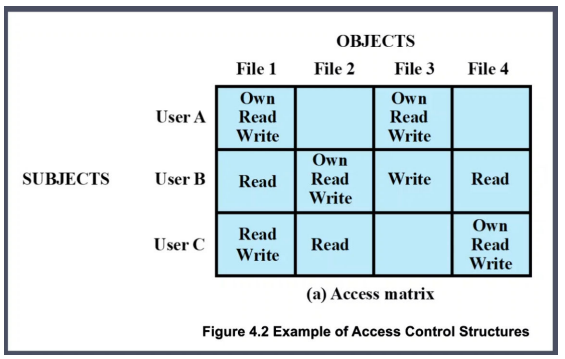
\includegraphics[width=10cm, keepaspectratio]{capitoli/policy/imgs/matrix_access_control.png}
      \caption{Esempio di Matrice di Controllo degli Accessi.}
\end{figure}

\noindent Nel caso in cui volessi avere accesso ad un file che non c’è, ci
sarebbe il file safe default di sistema, il default deve essere sempre safe. \\
Esistono anche altri metodi per mappare gli accessi (\textbf{più efficienti
      rispetto alle matrici}), come le \textbf{Access Control List} e le \textbf{Capability
      List}. Rispetto alle Access Control Matrix sono meno costose perché non
contengono coppie riga/colonna vuote e di conseguenza inutili. Sono utilizzate
in genere per mappare appunto l’Access Control Matrix.

\begin{figure}[H]
      \centering
      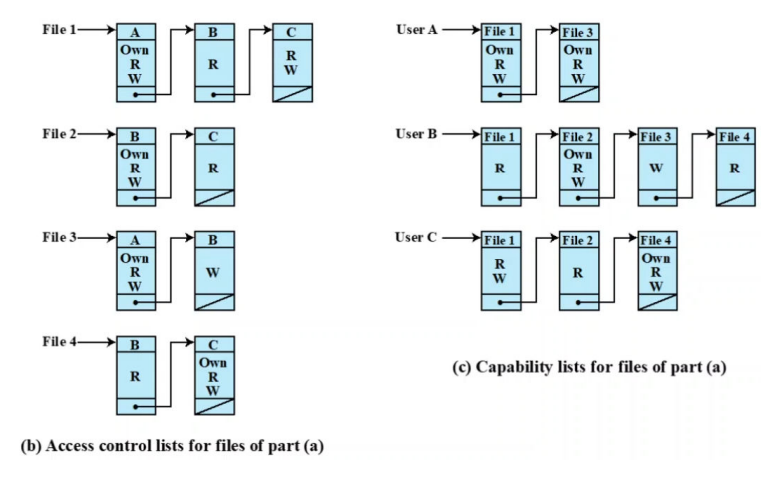
\includegraphics[width=12cm, keepaspectratio]{capitoli/policy/imgs/matrix_access_control2.png}
      \caption{ Access Control List e Capability List.}
\end{figure}
\noindent Solitamente può accadere che, quando la matrice di accesso è sparsa,
viene implementata tramite decomposizione in uno dei due modi.\\
\begin{itemize}
      \item La matrice può essere decomposta per colonne, ottenendo liste di
            controllo degli accessi (ACL). Per ogni oggetto, una ACL elenca gli utenti
            e i loro diritti di accesso consentiti. L'ACL può contenere una voce di
            default, o pubblica. Questo permette agli utenti che non sono
            esplicitamente elencati come aventi diritti speciali di avere un insieme
            predefinito di diritti. L'insieme predefinito di diritti dovrebbe sempre
            seguire la regola del minimo privilegio o dell'accesso in sola lettura, a
            seconda del caso. Gli elementi della lista possono includere sia utenti
            individuali che gruppi di utenti. Quando si vuole determinare quali
            soggetti hanno quali diritti di accesso a una particolare risorsa, le ACL
            sono convenienti, perché ogni ACL fornisce le informazioni per una data
            risorsa. Tuttavia, questa struttura di dati non è conveniente per
            determinare i diritti di accesso disponibili per un utente specifico.
      \item La decomposizione per righe produce i capability ticket. Un
            capability specifica gli oggetti e le operazioni autorizzate per un
            particolare utente. Ogni utente ha un certo numero di ticket e può essere
            autorizzato a prestarli o darli ad altri. Poiché i ticket possono essere
            dispersi nel sistema, essi presentano un maggiore problema di sicurezza
            rispetto alle liste di controllo degli accessi. L'integrità del biglietto
            deve essere protetta e garantita (di solito dal sistema operativo). In
            particolare, il biglietto deve essere non falsificabile. Questi biglietti
            dovrebbero essere tenuti in una regione di memoria inaccessibile agli
            utenti.  Gli aspetti convenienti e scomodi dei biglietti di capacità sono
            l'opposto di quelli delle ACL:
            \begin{itemize}
                  \item è facile determinare l'insieme dei diritti di accesso
                        che un dato utente ha,
                  \item ma è più difficile determinare l'elenco degli utenti con
                        diritti di accesso specifici per una risorsa specifica.
            \end{itemize}
\end{itemize}